\chapter{RZ- und IT-Management}

\section{Sie kennen die wichtigsten IT-Betriebsprozesse und
	verstehen die Bedeutung des IT-Betriebs für ein
	Unternehmen.}

Es stellt sich die Frage mit was IT-Unternehmen ihr Geld verdienen:
\begin{itemize}
	\item \textbf{IBM}\\
	Softwarelizenzen von Software, welche IBM entwickelt hat. Dabei leisten sie auch Beratung und Services. Der grösste Teil
	des Hardware-Geschäft wurde an Lenovo verkauft. Sie verkaufen jedoch noch Mainframes und Disk-Subsysteme. Ausserdem
	wohl die grösste Forschung für die IT.
	\item \textbf{HP}\\
	Vorallem im Hardware Geschäft. Marktführer im Server-Hardware Bereich. Aber auch noch Hersteller von Drucker, Notebooks,
	Desktop-PC.
	\item \textbf{Microsoft}\\
	Softwarentwicklung. Services werden durch zertifizierte Partner erledigt.
	\item \textbf{Accenture und AdNovum}\\
	Die IT Consulting Firmen der Schweiz (Beratungsbusiness).
	\item \textbf{Swisscom IT-Services}\\
	Betreiben Software. Sie entwickeln nicht Software - es ist ein anderes Geschäft als es ein Software-Entwicklungsunternehmen hat.
\end{itemize}

Was macht die IT-Abteilung in einer solchen Unternehmung?
\begin{itemize}
	\item Mittels IT-Services werden die Geschäftsprozesse (Kernprozesse) unterstützt. Die Folge daraus ist, dass man den Umsatz steigern möchte oder Kosten senken.
	\item Nehmen Anforderungen auf und ENTWICKELN Software. Klassische Softwareentwicklung. Dazu gehört auch Applikations-Einkauf.
	\item 'Entwickelte' Software müssen BETRIEBEN werden
\end{itemize}

MEP Frage: Was ist der Zweck der IT im unternehmen:
\label{zweck-der-it-im-unternehmen}
Die IT stellt IT Services zur Verfügung, welche die Kernprozesse des Unternehmens unterstützen. Mittels Entwicklung und/oder Betrieb von Software.

\begin{figure}[h!]
	\centering
	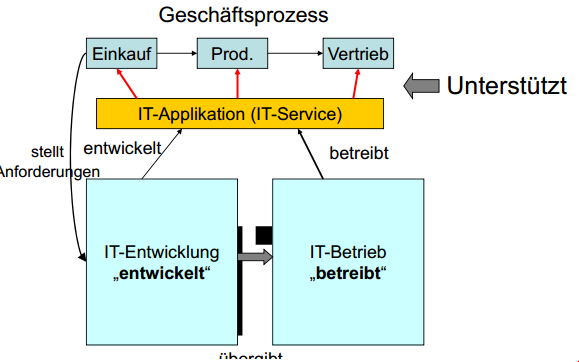
\includegraphics{fig/zweck-der-it}
	\caption{Zweck der IT}
\end{figure}

\textbf{IT-Betrieb}\\
Ziel: Keine Downtime. Es gibt auch partial Downtime, da ist nicht das ganze System down. Ziel sollte es schon sein, dass man eine Up-Time von 99.5 Prozent erreicht. Folgendes braucht es für eine stabile und hochverfügbare IT-Produktion: Hochstehende Applikationsentwicklung, QS und Kontrolle, Infrastruktur, Aufbau-Organisation, IT-Betriebsprozesse.

IT-Betrieb kann man in drei Bereiche unterteilen: 

\begin{itemize}
	\item Normal Operation (Daily Business)
	\item Change Operation (Ständige Neu-Entwicklung, Hardware ausbauen, grösste Fehlerquelle)
	\item Problem Operation (Es gibt immer Probleme)
\end{itemize}

Betriebsprozesse in IT Abteilungen:

Service Level Mgmt. (Vereinbarung über Services - Verfügbarkeit), IT-Service Continuity Mgmt. (Vorsorgemassnahmen: Planung bei Notfall), Architektur und Standards, Platform Mgmt.

Storage-Mgmt (Backup/Recovery), Monitoring, Change-Mgmt. (Planung von Änderungen),  Incident-/Problem Mgmt., SW/HW Deployment, Service/Help Desk

Configuration Mgmt. (Verwaltung von Hardware-Artefakte), Capacity Mgmt. (Prüfen ob man genügend Storage und CPU hat und Beschaffung Hardware und Software), Performance and Availability Mgmt., Financial Mgmt. (Services verrechnen, IT als Dienstleister innerhalb des Unternehmens), Supply Mgmt.

\section{Sie kennen den Incident-Management Prozesse und
	können Key Performance Indikatoren und Critical Success
	Factors erläutern.}
tbd